\begin{abcliste}
\abc Anfangszustand A: $(V_1, p_1)$. Die isotherme Kompression führt auf der Hyperbel $p\,V = p_1V_1$ nach B: $(V_1/2,\ 2\,p_1)$. Die isobare Expansion führt nach C: $(V_1,\ 2\,p_1)$. Zurück nach A geht es bei konstantem Volumen (isochor), der Druck halbiert sich. Der Prozess läuft im Uhrzeigersinn, das Gas gibt also netto Arbeit ab.
\begin{center}
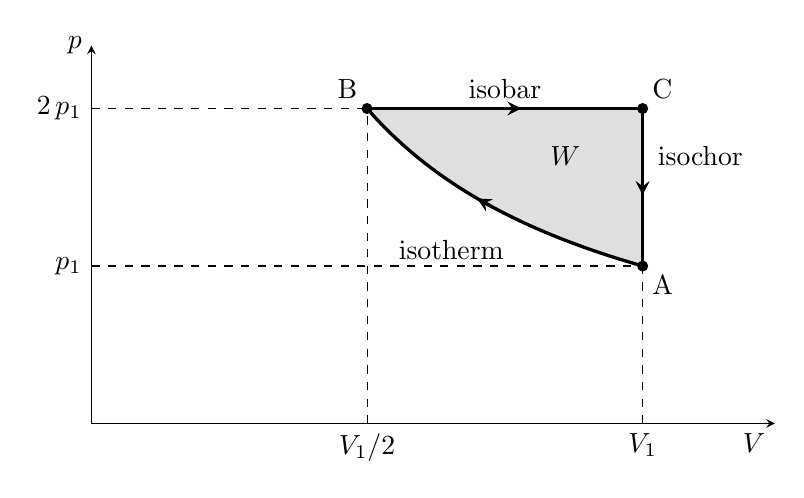
\begin{tikzpicture}[>=stealth, x=1.4cm, y=1cm]
 \fill[gray!25] (2.5,4) -- (5,4) -- (5,2) -- plot[domain=5:2.5, samples=40] (\x,{10/\x}) -- cycle;
 \draw[->] (0,0) -- (6.2,0) node[below left] {$V$};
 \draw[->] (0,0) -- (0,4.8) node[left] {$p$};
 \draw[very thick] plot[domain=2.5:5, samples=40] (\x,{10/\x});
 \draw[very thick] (2.5,4) -- (5,4) -- (5,2);
 \draw[->, very thick] (3.62,{10/3.62}) -- (3.5,{10/3.5});
 \draw[->, very thick] (3.6,4) -- (3.9,4);
 \draw[->, very thick] (5,3.1) -- (5,2.9);
 \draw[dashed] (2.5,0) node[below] {$V_1/2$} -- (2.5,4);
 \draw[dashed] (0,4) node[left] {$2\,p_1$} -- (2.5,4);
 \draw[dashed] (0,2) node[left] {$p_1$} -- (5,2);
 \draw[dashed] (5,0) node[below] {$V_1$} -- (5,2);
 \fill (5,2) circle (2pt) node[below right] {A};
 \fill (2.5,4) circle (2pt) node[above left] {B};
 \fill (5,4) circle (2pt) node[above right] {C};
 \node at (4.3,3.4) {$W$};
 \node[anchor=west] at (2.7,2.2) {isotherm};
 \node[above] at (3.75,4) {isobar};
 \node[anchor=west] at (5.05,3.4) {isochor};
\end{tikzpicture}
\end{center}

\abc Die vom Gas verrichtete Arbeit in den drei Schritten:
\begin{itemize}
\item A$\to$B (isotherm, $p = p_1V_1/V$): $W_\text{AB} = \int_{V_1}^{V_1/2} \frac{p_1V_1}{V}\,\mathrm{d}V = -p_1V_1\ln 2$
\item B$\to$C (isobar bei $2\,p_1$): $W_\text{BC} = 2\,p_1\left(V_1-\frac{V_1}{2}\right) = p_1V_1$
\item C$\to$A (isochor): $W_\text{CA} = 0$
\end{itemize}
Pro Zyklus gibt das Gas die Arbeit
\begin{align}
 W &= W_\text{AB}+W_\text{BC}+W_\text{CA} = \result{\WkF}
\end{align}
ab. Sie entspricht der vom Kreisprozess umschlossenen Fläche.

\abc Mit $V_1 = \VaO$ und $p_1 = \paO$:
\begin{align}
 W &= \WkF = \pa\cdot\Va\cdot\left(1-\ln 2\right) = \Wk \approx \result{\WkP{0}{2}}
\end{align}
\end{abcliste}
